
%=========================================================================
% Start of first day of vectors in 3D
%=========================================================================
\preClass{Introduction to Vectors in Three Dimensions.}

\begin{problem}
  \item Determine the distance between the points $P(2,4)$ and $Q(-1,5)$.

    \vfill
    \vfill

\item Determine a way to express the point $P$ shown in the diagram below as the sum of
the $\vec{\imath}$, $\vec{\jmath}$, and $\vec{k}$ vectors.

  \tdplotsetmaincoords{60}{100}
  \begin{tikzpicture}[tdplot_main_coords]
    % Draw the coordinates
    \coordinate (O) at (0, 0, 0);
    \draw[->] (O) -- +(4, 0, 0) node[font = \small, pos = 1.1] {\(x\)} coordinate (X);
    \draw[->] (O) -- +(0, 4, 0) node[font = \small, pos = 1.1] {\(y\)} coordinate (Y);
    \draw[->] (O) -- +(0, 0, 4) node[font = \small, pos = 1.1] {\(z\)} coordinate (Z);
    %
    % Draw the unit vectors
    \draw[very thick,blue,->] (0,0,0) -- (1,0,0) node[font=\small,pos=1.7,anchor=south west] {$\hat{\imath}$};
    \draw[very thick,blue,->] (0,0,0) -- (0,1,0) node[font=\small,pos=0.9,anchor=south west] {$\hat{\jmath}$};
    \draw[very thick,blue,->] (0,0,0) -- (0,0,1) node[font=\small,pos=0.9,anchor=south east] {$\hat{k}$};
    %
    % Draw a point in space
    \node[draw=none,shape=circle,fill, inner sep=2pt] (d1) at (2,1,3){};  % circle
    \node[font=\small,anchor=south] at (d1) {P};  % label
    \draw[thin,red,dashed] (2,0,0) -- (2,1,0) node[font=\small,pos=0.5,anchor=north] {1};
    \draw[thin,red,dashed] (0,1,0) -- (2,1,0) node[font=\small,pos=0.25,anchor=north west] {2};
    \draw[thin,red,dashed] (2,1,0) -- (2,1,3) node[font=\small,pos=0.75,anchor=west] {3};
  \end{tikzpicture}

  \vfill

\end{problem}


\actTitle{Vectors in Three Dimensions}
\begin{problem}
\item Make a sketch of the coordinate axes in three dimensions.

  \vfill
  \begin{subproblem}
      \item Make sure to label the axes.
      \item Add the point $P(4,1,2)$ to your plot.
      \item Add the point $Q(1,4,0)$ to your plot.
      \item Add the vector $PQ$ to your plot.
  \end{subproblem}
  \clearpage

\item A point, $P$, has coordinates $(x,y,z)$ as shown in the diagram below.
  The point $Q$ is directly beneath $P$ at $(x,y,0)$.

\tdplotsetmaincoords{60}{100}
\begin{tikzpicture}[tdplot_main_coords]
  % Draw the coordinates
  \coordinate (O) at (0, 0, 0);
  \draw[->] (O) -- +(4, 0, 0) node[font = \small, pos = 1.1] {$x$} coordinate (X);
  \draw[->] (O) -- +(0, 4, 0) node[font = \small, pos = 1.1] {$y$} coordinate (Y);
  \draw[->] (O) -- +(0, 0, 4) node[font = \small, pos = 1.1] {$z$} coordinate (Z);
  \node[font=\small,anchor=east] at (0,0,0) {$O$};
  %
  % Draw a point in space
  \draw[->] (O) -- +(3, 2, 4) node[font = \small, pos = 1.1] {} coordinate (P);
  \node[font=\small,anchor=south] at (P) {P};  % label
  \draw[thin,red,dashed]  (3,0,0) -- (3,2,0) node[font=\small,pos=0.5,anchor=north] {$x$};
  \draw[thin,red,dashed]  (0,2,0) -- (3,2,0) node[font=\small,pos=0.25,anchor=north west] {$y$};
  \draw[thin,red,dashed]  (3,2,0) -- (3,2,4) node[font=\small,pos=0.75,anchor=west] {$z$};
  \draw[thin,blue,dashed] (0,0,0) -- (3,2,0) node[font=\small,pos=0.5,anchor=west] {$h$};
  \draw[thin,blue] (2.8,1.8,0) -- (2.8,1.8,.4) -- (3,2,.4);
  \node[draw=none,shape=circle,fill, inner sep=2pt] (Q) at (3,2,0) {};
  \node[font=\small,anchor=north] at (Q) {Q};
\end{tikzpicture}

\begin{subproblem}
  \item Determine the distance, $h$, from the origin, $O$, to the point $Q$.
    \vfill
  \item Determine the distance between $Q$ and $P$.
    \vfill
  \item Determine the distance between $P$ and the origin in terms of $x$, $y$, and $z$. (Hint: Draw a side view of the triangle $OQP$.
    \vfill
\end{subproblem}

\clearpage

\item Determine the distance between two points, $P(x_0,y_0,z_0)$ and $Q(x_1,y_1,z_1)$.
   (Hint: The distance between the points is the same as the length of the vector $\vec{PQ}$.)

   \vfill

 \item Determine the formula for the set of all points that are a distance of 2 m from the point $Q(2,-1,5)$.

  \vfill

  \item What is another way to describe the set of all points a distance of 2m from the point  $Q(2,-1,5)$?

\end{problem}


\postClass

\begin{problem}
\item Briefly state two ideas from today's class.
  \begin{itemize}
  \item
  \item
  \end{itemize}
\item
  \begin{subproblem}
    \item
  \end{subproblem}
\end{problem}


%=========================================================================
% Start of second day of vectors in 3D
%=========================================================================
\preClass{Length of a Vector}

\begin{problem}
\item Sketch and label the vectors $\vec{u}=2\vec{\imath}+3\vec{\jmath}$ and
      $\vec{v}=-\vec{\imath}+2\vec{\jmath}$ on the diagram below.

    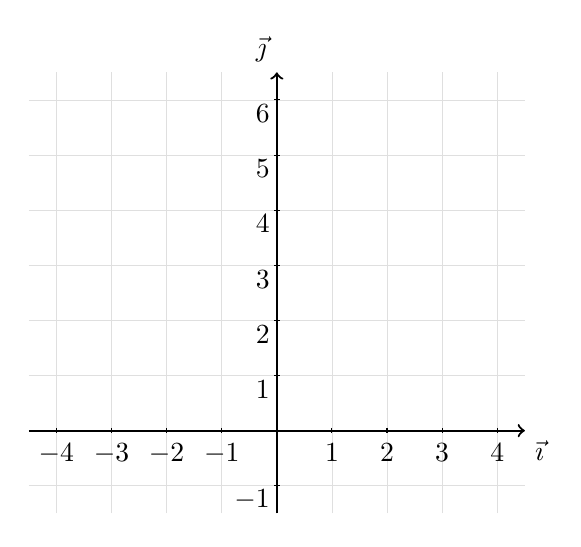
\begin{tikzpicture}[y=0.7cm, x=0.7cm,font=\sffamily]
      % ticks
      \draw[step = 1, gray, very thin,opacity=0.25] (-4.5, -1.5) grid ( 4.5, 6.5);
      % axis
      \draw[thick,->] (-4.5,0) -- coordinate (x axis mid) (4.5,0) node[anchor = north west] {$\vec{\imath}$};
      \draw[thick,->] (0,-1.5) -- coordinate (y axis mid) (0,6.5) node[anchor = south east] {$\vec{\jmath}$};
      \foreach \y in {-1,1,2,...,6} {
        \draw (1pt, \y) -- (-1pt, \y) node[anchor = east,yshift=-5,xshift=2] {$\y$};
      }
      \foreach \x in {-4,-3,...,-1,1,2,3,4} {
        \draw (\x,1pt) -- (\x,-1pt) node[anchor = north ] {$\x$};
      }
    \end{tikzpicture}

\item Add a sketch the vector $\vec{u}+\vec{v}$ to your plot. Express the resultant in component form.

    \vfill

\item Add a sketch the vector $\vec{u}-\vec{v}$ to your plot. Express the resultant in component form.

    \vfill

\item Determine the lengths of the vectors $\vec{u}$ and $\vec{v}$.

  \vfill

\end{problem}


\actTitle{Length of Vectors in Three Dimensions}
\begin{problem}
\item Sketch and label the vectors $\vec{u}=1\vec{\imath}+2\vec{\jmath}$ and
      $\vec{v}=-3\vec{\imath}-2\vec{\jmath}$ on the diagram below.

  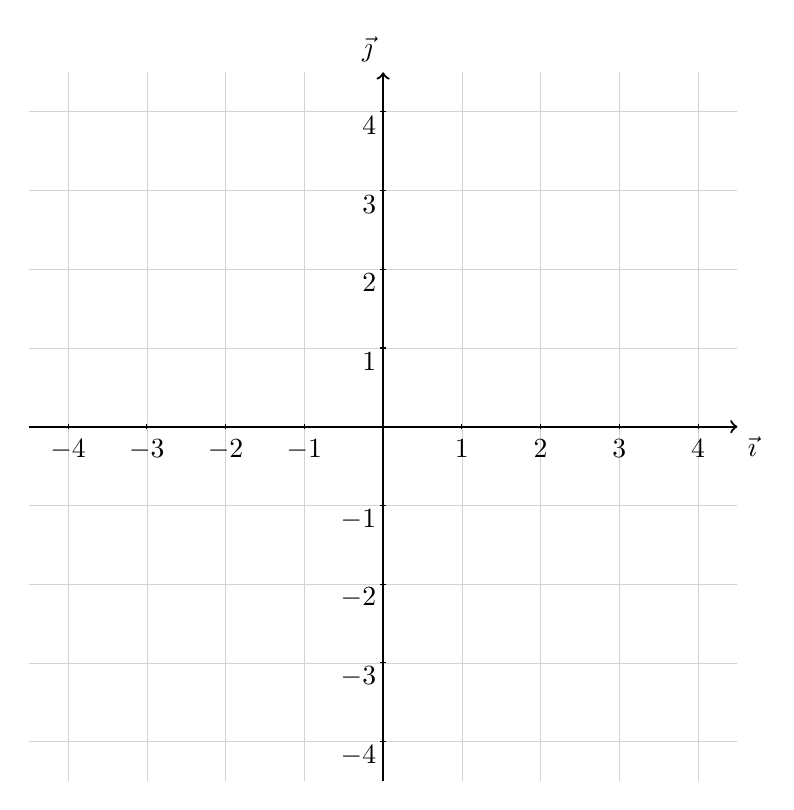
\begin{tikzpicture}[y=1.0cm, x=1.0cm,font=\sffamily]
    % ticks
    \draw[step = 1, gray, very thin,opacity=0.35] (-4.5, -4.5) grid ( 4.5, 4.5);
    % axis
    \draw[thick,->] (-4.5,0) -- coordinate (x axis mid) (4.5,0) node[anchor = north west] {$\vec{\imath}$};
    \draw[thick,->] (0,-4.5) -- coordinate (y axis mid) (0,4.5) node[anchor = south east] {$\vec{\jmath}$};
    \foreach \y in {-4,-3,...,-1,1,2,3,4} {
      \draw (1pt, \y) -- (-1pt, \y) node[anchor = east,xshift=2pt,yshift=-5pt] {$\y$};
    }
    \foreach \x in {-4,-3,...,-1,1,2,3,4} {
      \draw (\x,1pt) -- (\x,-1pt) node[anchor = north] {$\x$};
    }
  \end{tikzpicture}

  \begin{subproblem}
      \item Determine the magnitudes of the two vectors.
      \vfill
%      \item What are the angles between the vectors and the $\vec{\imath}$ axis.
%      \vfill
      \item Add a sketch of the vectors $-2\vec{u}$ and $\frac{1}{2}\vec{v}$ to the plot.
      %In each case what happens to the angle between the vector and the $\vec{\imath}$ axis?
      What is the relationship between the new vectors and the original vectors?
      \vfill
      \item Is it possible to find a value of $k$ so that $\vec{u}=k\vec{v}$? (Explain how you arrived at your conlcusion.)
      \vfill
  \end{subproblem}

\clearpage

\item Suppose that you have two vectors, $\vec{u}=u_1 \vec{\imath}+u_2\vec{\jmath}$ and $\vec{v}=v_1 \vec{\imath}+v_2\vec{\jmath}$.
      Assume that $u_1$, $u_2$, $v_1$, and $v_2$ are constants.

  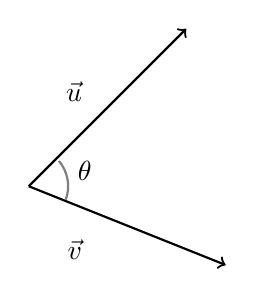
\begin{tikzpicture}[y=1.0cm, x=1.0cm,font=\sffamily]
    % ticks
    \draw[thick,->] (0,0) -- (2.5,-1.0);
    \draw[thick,->] (0,0) -- (2.0,2.0);
    \node[anchor=west] at (0.5,0.2) {$\theta$};
    \node[anchor=east] at (0.8, 1.2) {$\vec{u}$};
    \node[anchor=east] at (0.8,-0.8) {$\vec{v}$};
    \draw[thick,gray] ++(-20:0.5) arc (-20:40:0.5) ;
  \end{tikzpicture}

  \begin{subproblem}
    \item Add a sketch of the vector $\vec{u}-\vec{v}$ to the sketch above.
    \item Use the law of cosines to relate $\vec{u}$, $\vec{v}$, and $\vec{u}-\vec{v}$.
      \vspace{4em}
    \item Use the definitions of $\vec{u}$ and $\vec{v}$ above to determine the algebraic value of
    \begin{eqnarray*}
      \frac{1}{2} \left[ \|\vec{u}\|^2 +  \|\vec{v}\|^2 -  \|\vec{u}-\vec{v}\|^2\right].
    \end{eqnarray*}
    \vfill
    \item Determine a formula for the cosine of the angle between two vectors.
    \vspace{4em}
  \end{subproblem}

\end{problem}


\postClass

\begin{problem}
\item Briefly state two ideas from today's class.
  \begin{itemize}
  \item
  \item
  \end{itemize}
\item
  \begin{subproblem}
    \item
  \end{subproblem}
\end{problem}

%=========================================================================
% Start of day on vector components
%=========================================================================
\preClass{Unit Vector}

\begin{problem}
\item The following questions refer to the vector
\begin{eqnarray*}
  \vec{u} & = & 3 \vec{\imath} + 1 \vec{\jmath}.
\end{eqnarray*}
\begin{subproblem}
    \item Make a sketch of the vector including the coordinate axes.
    \vfill
    \item Add a sketch of the vector $\half \vec{u}$ to your plot above.
    \item Determine the length of the vector $\vec{u}$.
    \vfill
    \item Determine values of $k$ so that the vector $k \vec{u}$ has length one.
    \vfill
\end{subproblem}
\end{problem}


\actTitle{Vector Components}
\begin{problem}
  \item Given the vector $\vec{w}=3\vec{\imath} +4 \vec{\jmath}$ answer the following questions.

    \begin{subproblem}
        \item Make a sketch of a set of axes and the vector.
        \vfill
        \item Determine another vector $\hat{w}$ that has a length of one and points in the same direction of $\vec{w}$.
        \vfill
        \item Determine another vector, $\vec{r}$, that has length 5 and points in the opposite direction as $\vec{w}$.
        \vfill
    \end{subproblem}

    \clearpage

  \item The vectors $\vec{u}$ and $\vec{v}$ are shown in the diagram below:

    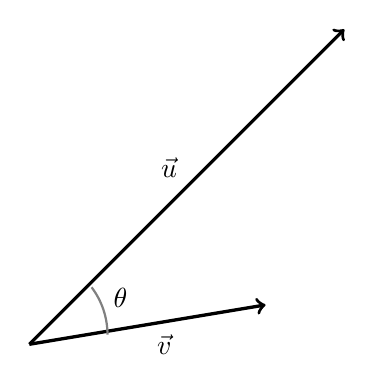
\begin{tikzpicture}[y=1.0cm, x=1.0cm,font=\sffamily]
    \draw[black,very thick,->] (0,0) -- (4,4);
    \node[black,anchor=south east] at (2,2) {$\vec{u}$};
    \draw[black,very thick,->] (0,0) -- (3,0.5);
    \node[black,anchor=north west] at (1.5,.25) {$\vec{v}$};
    \draw[thick,gray] (7:1.0) arc (0:37:1.0) ;
    \node[black] at (27:1.3) {$\theta$};
    \end{tikzpicture}

  \begin{subproblem}
    \item Extend a dotted line on the diagram along $\vec{v}$ in the direction of $\vec{v}$
    \item Draw a line from the top of $\vec{u}$ down to the dotted line so that the line is perpindicular to the dotted line.
    \item You should now see a triangle in the diagram. What is the length of the hypotenuse of the triangle?
      \vfill
    \item What is the length of the side opposite to the angle $\theta$?
      \vfill
    \item What is the length of the side adjacent to the angle $\theta$?
      \vfill

      \clearpage

    \item What is the value of $\vec{u}\cdot\vec{v}$ in terms of $\|\vec{u}\|$, $\|\vec{v}\|$, and $\theta$?
      \vfill

    \item Determine the length of the side adjacent to the angle $\theta$ in terms of the previous dot product.
      \vfill

    \item Determine the unit vector in the direction of $\vec{v}$.
      \vfill

    \item Determine the vector in the direction of $\vec{v}$ whose length is equal to the length of the side adjacent to the angle $\theta$.
      \vfill

  \end{subproblem}

  \clearpage

  \item If $\vec{u}=3\vec{\imath}+2\vec{\jmath}$ and $\vec{v}=1\vec{\imath}+1\vec{\jmath}$ determine the component of $\vec{u}$ that is in the direction of $\vec{v}$.
    \vfill

\end{problem}

\postClass

\begin{problem}
\item Briefly state two ideas from today's class.
  \begin{itemize}
  \item
  \item
  \end{itemize}
\item
  \begin{subproblem}
    \item
  \end{subproblem}
\end{problem}


%=========================================================================
% Start of activity on the cross product
%=========================================================================
\preClass{The Area of a Parallelogram}

\begin{problem}
\item Determine the area of the parallelogram shown below. The area
  should be in terms of $a$, $b$, and $\theta$.

  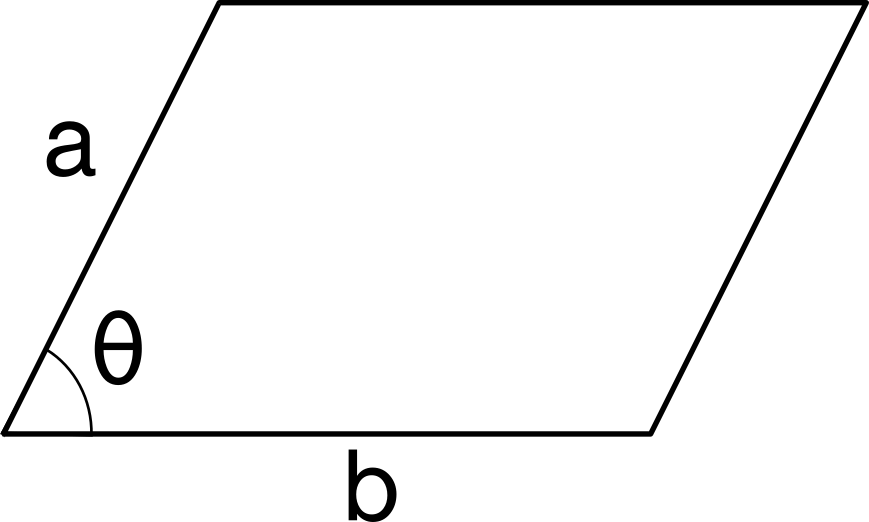
\includegraphics[width=5cm]{../semI/ink/week11/parallelogram}

  \vfill

\item Expand the expression
  \begin{eqnarray*}
    \left( a + b \right) \cdot \left( c + d \right)
  \end{eqnarray*}
  where ``$\cdot$'' is scalar multiplication.

  \vfill

\end{problem}


\actTitle{The Cross Product}
\begin{problem}
\item The cross product of two vectors, $\vec{u}\times\vec{v}$, is
  derived by first defining  the following identities:
  \begin{eqnarray*}
    \vec{\imath} \times \vec{\jmath} & = & \vec{k}, \\
    \vec{\jmath} \times \vec{k} & = & \vec{\imath}, \\
    \vec{k} \times \vec{\imath} & = & \vec{\jmath}, \\
    \vec{u} \times \vec{u} & = & 0 \vec{\imath}, \\
    \vec{u} \times \vec{v} & = & - \vec{v} \times \vec{u}.
  \end{eqnarray*}
  \begin{subproblem}
  \item For the first three identities above make a sketch to
    demonstrate the relationships.
    \vfill

    \item The result of $\vec{\imath}\times\vec{\jmath}$ is what kind of thing?
    \sideNote{Is it a scalar or a vector?}
    \vspace{3em}

    \item The result of $\vec{\imath}\cdot\vec{\jmath}$ is what kind of thing?
    \sideNote{Is it a scalar or a vector?}
    \vspace{3em}

    \clearpage

  \item Suppose that
    \begin{eqnarray*}
      \vec{u} & = & u_1 \vec{\imath} + u_2 \vec{\jmath}
    \end{eqnarray*}
    and
    \begin{eqnarray*}
      \vec{v} & = & v_1 \vec{\imath} + v_2 \vec{\jmath}.
    \end{eqnarray*}
    Use the definitions above and assume that the cross product obeys
    the distributive rule to derive a general formula for the cross
    product, $\vec{u}\times\vec{v}$.
    \vfill
    \vfill

    \clearpage

  \item Determine the vector $\left(2 \vec{\imath} + 2\vec{\jmath}\right) \times \left(4 \vec{\imath}\right)$.
    \vfill

  \item Determine the vector $\left( 4 \vec{\imath} \right)  \times  \left( 2 \vec{\imath} + 2\vec{\jmath}\right)$.
    \vfill

  \item What are the directions of the resulting vectors from the cross product with respect to the original vectors?
    \vspace{2em}

    \clearpage

  \item Suppose that
    \begin{eqnarray*}
      \vec{u} & = & u_1 \vec{\imath} + u_2 \vec{\jmath} + u_3 \vec{k}
    \end{eqnarray*}
    and
    \begin{eqnarray*}
      \vec{v} & = & v_1 \vec{\imath} + v_2 \vec{\jmath} + v_3 \vec{k}.
    \end{eqnarray*}
    Use the definitions above and assume that the cross product obeys
    the distributive rule to derive a general formula for the cross product.
    \vfill

  \end{subproblem}
\end{problem}


\postClass

\begin{problem}
\item Briefly state two ideas from today's class.
  \begin{itemize}
  \item
  \item
  \end{itemize}
\item
  \begin{subproblem}
    \item
  \end{subproblem}
\end{problem}

%=========================================================================
% Start of day on determinants
%=========================================================================
\preClass{Solving Linear Systems}

\begin{problem}
\item In the steps below determine the solution to the system of equations given by
\begin{eqnarray*}
  \begin{array}{lcl}
    3x + 2y & = & 5, \\
    c \cdot x + 4y & = & 6,
  \end{array}
\end{eqnarray*}
where $c$ is a constant.
\begin{subproblem}
  \item Use the first equation to solve for $y$ as a function of $x$.
    \vfill
  \item Substitute your value for $y$ into the second equation.
    \vfill
  \item Solve the new equation for $x$.
    \vfill
  \item Use the previous expression to determine a value for $c$ for which it is not possible to solve the system.
    \vfill
\end{subproblem}
\end{problem}


\actTitle{Determinants}
\begin{problem}
\item We want to determine the conditions that are necessary for a system of linear
  equations to have a solution. Two general, constant coefficient equations are defined.
  In the steps below determine the solution to the system of equations given by
\begin{eqnarray*}
  \begin{array}{lcl}
    a \cdot x + b \cdot y & = & r_1, \\
    c \cdot x + d \cdot y & = & r_2,
  \end{array}
\end{eqnarray*}
where $a$, $b$, $c$, $d$, $r_1$, and $r_2$ are constants.
\begin{subproblem}
  \item Use the first equation to solve for $y$ as a function of $x$.
    \vfill
  \item Substitute your value for $y$ into the second equation.
    \vfill
  \item Solve the new equation for $x$.
    \vfill
  \item Determine the relationship that insures that there is a unique solution to the system.
    \vfill
\end{subproblem}

  \clearpage

\item Without solving the following system of equations, use your previous result as a check to determine if it is possible to determine a unique solution to the following system of equations:
\begin{eqnarray*}
  \begin{array}{lcl}
     4x - 2y & = & 5, \\
    -2x + y & = & 8.
  \end{array}
\end{eqnarray*}

  \vspace{4em}

\item Solve the following system directly without using the previous formula. Can a solution be found?
\begin{eqnarray*}
  \begin{array}{lcl}
     4x - 2y & = & 5, \\
    -2x + y & = & 8.
  \end{array}
\end{eqnarray*}

\vfill
\clearpage

\item Solve the following system directly without using the previous formula. Can a solution be found?
\begin{eqnarray*}
  \begin{array}{lcl}
     4x - 2y & = & 6, \\
    -2x + y & = & -3.
  \end{array}
\end{eqnarray*}

\vfill

\item What makes the two previous examples different from one another and why can one be solved but not the other?
  \vspace{4em}


\end{problem}


\postClass

\begin{problem}
\item Briefly state two ideas from today's class.
  \begin{itemize}
  \item
  \item
  \end{itemize}
\item
  \begin{subproblem}
    \item
  \end{subproblem}
\end{problem}


%=========================================================================
% Start of first day of lines and parameterization of a line
%=========================================================================
\preClass{Lines}

\begin{problem}
\item A turtle starts at the origin. It moves at a constant speed of 1
  meters per minute. It is facing in the direction of the positive $x$-axis.
  Determine its position at any time.

  \vfill

\item A turtle starts at the origin. It moves at a constant speed of 1
  meters per minute. It is facing in a direction $\frac{\pi}{2}$
  radians from the $x$-axis and is moving along the positive $y$-axis.
  Determine its position at any time.

  \vfill


\end{problem}


\actTitle{Parameterization of a Line}
\begin{problem}

  \item A turtle starts at the origin. It moves at a constant speed of 2
    meters per minute. It is facing in a direction $\frac{\pi}{4}$
    radians from the $x$-axis and is moving in the first
    quadrant.
    \begin{subproblem}
      \item Draw a picture of the $x-y$ plane with the direction of movement as a vector.
         Express its direction of movement as a vector in terms of $\hat{\imath}$ and $\hat{\jmath}$.
        \vfill
      \item What is its position after one minute?
        \vfill
      \item What is its position after two minutes?
        \vfill
      \item What is its position after $t$ minutes?
        \vfill
    \end{subproblem}
    \vfill

  \clearpage

  \item At $t=0$s an object is located at the point $\hat{\imath}+5\hat{\jmath}-3\hat{k}$  and is
  moving at a constant rate. After one minute its displacement is $4\hat{\imath}-2\hat{\jmath}+6\hat{k}$
  away from its initial position. (All distances are in meters.)
  Determine its position at any time.

    \vfill

  \item Suppose that an object's position is given by the formula you
    derived in the previous question. Determine its velocity.
    \sideNote{Determining velocity from position is no different in the
      context of vectors.}

  \vfill

  \clearpage

\item Given the equation of a line $\vec{r}(t)=\vec{r}_0 + t \vec{v}_0$ where the vectors $\vec{r}$ and $\vec{v}_0$ are constants. Determine $\frac{d}{dt}\vec{r}(t)$.
  \vfill

\item Given that an object has a constant velocity,  $\vec{v}_0$, determine its position.
  \vfill

\end{problem}


\postClass

\begin{problem}
\item Briefly state two ideas from today's class.
  \begin{itemize}
  \item
  \item
  \end{itemize}
\item
  \begin{subproblem}
    \item
  \end{subproblem}
\end{problem}

%=========================================================================
% Start of activity on distance between a point and a line
%=========================================================================
\preClass{How close is a point to a line?}

\begin{problem}
\item Make a sketch of a coordinate axes in the $x$ and $y$ directions.
  \vfill
\begin{subproblem}
  \item Mark the point $P(1,2)$ and $Q(3,1)$.
  \item What is the distance between the two points?
    \vspace{3em}
\end{subproblem}

\item Make a sketch of a coordinate axes in the $x$ and $y$ directions.
  \vfill
\begin{subproblem}
  \item Sketch the line $y=2$ and the point $P(1,3)$.
  \item What is the distance between the point and the line?
    \vspace{3em}
\end{subproblem}


\end{problem}


\actTitle{Distance between a point and a line}
\begin{problem}

\item Suppose $\vec{r}(t)$ is a line in space, and $P$ is a point in space.

  \tdplotsetmaincoords{60}{100}
  \begin{tikzpicture}[tdplot_main_coords]
    % Draw the coordinates
    \coordinate (O) at (0, 0, 0);
    \draw[->] (O) -- +(4, 0, 0) node[font = \small, pos = 1.1] {\(x\)} coordinate (X);
    \draw[->] (O) -- +(0, 4, 0) node[font = \small, pos = 1.1] {\(y\)} coordinate (Y);
    \draw[->] (O) -- +(0, 0, 4) node[font = \small, pos = 1.1] {\(z\)} coordinate (Z);
    %
    %
    % Draw a point in space
    \node[draw=none,shape=circle,fill, inner sep=2pt] (d1) at (4,3,1){};  % circle
    \node[font=\small,anchor=south] at (d1) {P};  % label
    % Draw a line in space
    \draw[very thick,blue] (1,-2,-2) -- (2,4,4) node[font=\small,pos=0.9,anchor=north west] {$\vec{r}(t)$};
  \end{tikzpicture}

  \begin{subproblem}
    \item Looking at the graph above, make a rough estimate for the point on $\vec{r}(t)$ that is closest to $P$. Mark it on the plot and call it $Q$.
    \item Draw a vector, call it $\vec{PQ}$, that starts at the point you made and ends at $P$.
    \item Mark an arbitrary point on the line, call it $S$.
    \item What is the relationship between $\vec{PQ}$ and $\vec{SQ}$?
      \vfill
    \item Identify and label the angle $\theta$ that is between $\vec{SQ}$ and $\vec{SQ}$.

    \clearpage

    \item Redraw the triangle that has $\vec{PQ}$, $\vec{SQ}$, and $\vec{SP}$. Draw it as if you are looking directly at it from the side.
      \vfill

    \item Which part of the triangle represents the distance between the point $P$ and the line? Determine the distance in terms of $\theta$ and $\vec{SP}$.
      \vfill

    \item Which is more appropriate to use here a dot product or a cross product. (We want to find the expression in the previous question!)
      \vfill

    \item Determine the appropriate dot or cross product that has the relevant term in it. Manipulate it to get the distance between the point and the line.
      \vfill

  \end{subproblem}

  \clearpage

  \item Determine the distance between the point $(4,3,1)$ and the line $\vec{r}(t)=\left(1\vec{\imath}-2\vec{\jmath}-2\vec{k}\right)+t\left(1\vec{\imath}+6\vec{\jmath}+6\vec{k}\right)$.
    \vfill

\end{problem}


\postClass

\begin{problem}
\item Briefly state two ideas from today's class.
  \begin{itemize}
  \item
  \item
  \end{itemize}
\item
  \begin{subproblem}
    \item
  \end{subproblem}
\end{problem}


%=========================================================================
% Start of activities on equations for planes
%=========================================================================
\preClass{Orthogonal vectors}

\begin{problem}
\item Suppose two vectors, $\vec{n}=0\vec{\imath}+0\vec{\jmath}+2\vec{k}$ and $\vec{u}$, and perpindicular to one another.
  \begin{subproblem}
    \item What must the value of the dot product, $\vec{n}\cdot\vec{u}$ of the two vectors be?
      \vfill
    \item Suppose that $\vec{u}=x\vec{\imath}+y\vec{\jmath}+z\vec{k}$.  What does that imply about the value of $z$?
      \vfill
    \item What restruction is there on the values of $x$ and $y$?
      \vfill
  \end{subproblem}
\end{problem}


\actTitle{Equation for a plane}
\begin{problem}
\item Suppose that $P$ is a point on a plane, and $\vec{n}$ is a vector that is perpendicular to the plane at the point $P$.

  \tdplotsetmaincoords{60}{100}
  \begin{tikzpicture}[tdplot_main_coords,fill opacity=.3]
    % Draw the coordinates
    \coordinate (O) at (0, 0, 0);
    \draw[->] (O) -- +(4, 0, 0) node[font = \small, pos = 1.1] {\(x\)} coordinate (X);
    \draw[->] (O) -- +(0, 4, 0) node[font = \small, pos = 1.1] {\(y\)} coordinate (Y);
    \draw[->] (O) -- +(0, 0, 4) node[font = \small, pos = 1.1] {\(z\)} coordinate (Z);
    %
    %
    % Draw a plane in space
    \filldraw[draw=red,fill=red!10,fill opacity=0.1]  (4,0,1) -- (4,3,2.5) -- (0,3,1.5) -- (0,0,0) -- cycle;
    % Draw a point in space
    \node[draw=none,shape=circle,fill, inner sep=2pt] (d1) at (2,2,1.5){};  % circle
    \node[font=\small,anchor=south west] at (d1) {P};  % label
    % Draw the normal vector
    \draw[->] (d1) -- +(-0.25,-0.5,1) node[font = \small,pos=1.4] {$\vec{n}$};
  \end{tikzpicture}

  \begin{subproblem}
    \item Mark and label a point $Q$ on the plane in the diagram above.
    \item What is the angle between the vector $\vec{PQ}$ and the vector $\vec{n}$?
      \vspace{3em}
    \item What can you say about the dot product and the cross product of the vectors $\vec{PQ}$ and $\vec{n}$? Which is an easier relationship to work with?
      \label{activity:planes:normalRelationship}
      \vfill

      \clearpage

    \item Assume that $P$ is a fixed point, $P=x_0\vec{\imath}+y_0\vec{\jmath}+z_0\vec{k}$, and $Q$ is any point in the plane, $Q=x\vec{\imath}+y\vec{\jmath}+z\vec{k}$.
      Determine the vector $\vec{PQ}$.
        \vfill
    \item Using the relationship from part \ref{activity:planes:normalRelationship}, determine a relationship that describes all points on the plane.
      \vfill
    \item Suppose that the point $P=3\vec{\imath}-1\vec{\jmath}+2\vec{k}$ is on a plane, and the vector $\vec{n}=-5\vec{\imath}+4\vec{\jmath}-1\vec{k}$ is perpendicular to the plane.
       Determine the equation for the plane.
       \vfill
       \vfill
  \end{subproblem}
\end{problem}


\postClass

\begin{problem}
\item Briefly state two ideas from today's class.
  \begin{itemize}
  \item
  \item
  \end{itemize}
\item
  \begin{subproblem}
    \item
  \end{subproblem}
\end{problem}





%%% Local Variables:
%%% mode: latex
%%% TeX-master: "labManual"
%%% End:
